\documentclass[tikz,border=2pt]{standalone}
\usepackage{amsmath,amssymb}
\usepackage{tikz}

\begin{document}
% Open: none of its boundary points belong to it (dashed rim). Closed: all of them do (solid rim).
% Neither: some do, some do not (half solid, half dashed).
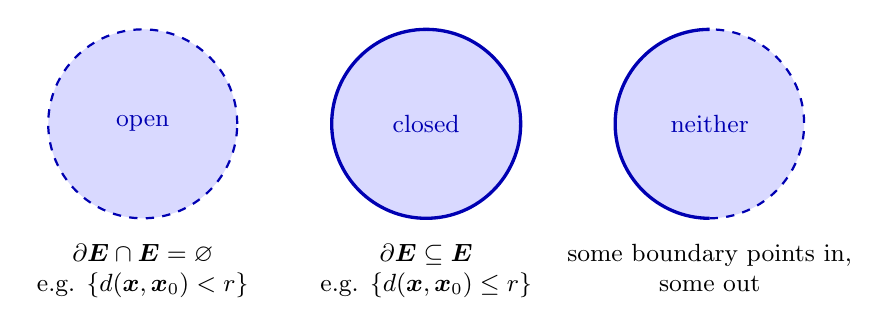
\begin{tikzpicture}[every node/.style={font=\small}]
	\fill[blue!15] (0,0) circle (1.2);
	\draw[blue!70!black, thick, dashed] (0,0) circle (1.2);
	\node[blue!70!black] at (0,0) {open};
	\node[anchor=north, align=center] at (0,-1.4) {$\partial\boldsymbol{E}\cap\boldsymbol{E}=\varnothing$\\ e.g. $\{d(\boldsymbol{x},\boldsymbol{x}_0)<r\}$};
	\begin{scope}[xshift=3.6cm]
		\fill[blue!15] (0,0) circle (1.2);
		\draw[blue!70!black, very thick] (0,0) circle (1.2);
		\node[blue!70!black] at (0,0) {closed};
		\node[anchor=north, align=center] at (0,-1.4) {$\partial\boldsymbol{E}\subseteq\boldsymbol{E}$\\ e.g. $\{d(\boldsymbol{x},\boldsymbol{x}_0)\le r\}$};
	\end{scope}
	\begin{scope}[xshift=7.2cm]
		\fill[blue!15] (0,0) circle (1.2);
		\draw[blue!70!black, very thick] (0,0) ++(90:1.2) arc (90:270:1.2);
		\draw[blue!70!black, thick, dashed] (0,0) ++(-90:1.2) arc (-90:90:1.2);
		\node[blue!70!black] at (0,0) {neither};
		\node[anchor=north, align=center] at (0,-1.4) {some boundary points in,\\ some out};
	\end{scope}
\end{tikzpicture}
\end{document}
